
\chapter{Anforderungserhebung}\label{sec:chapter5}
In diesem Kapitel werden die Anforderungen an den in Kapitel 6 folgenden Vergleich der imperativen und deklarativen Modellierung für SE-Prozessmodelle erhoben.

\section{Vergleichskriterien}\label{sec:chapter5:Vergleichskriterien}

Bisher gibt es nur wenige Arbeiten, welche sich mit deklarativen Prozessmodellierungssprachen und insbesondere mit dem Vergleich von imperativen und deklarativen Prozessmodellierungssprachen beschäftigen. Aus diesem Grund soll in der vorliegenden Arbeit ein Vergleich zwischen deklarativen und imperativen Prozessmodellierungssprachen im Kontext von Software-Engineering Prozessmodellen durchgeführt werden. Hierbei sollen die Unterschiede und Ähnlichkeiten der beiden Prozessmodellierungssprachen herausgearbeitet und deren Eignung für die Modellierung von unterschiedlich großen Prozessmodellen beurteilt werden. Weiterhin sollen die Stärken und Grenzen der beiden Modellierungssprachen aufgezeigt werden und es soll dadurch herausgefunden werden, ob eine der beiden Modellierungssprachen über eine bessere Eignung zur Modellierung verfügt als die andere \cite{list2006evaluation}.\newline
Hierfür sollen die imperativen und deklarativen Prozessmodelle, welche für die drei Software-Engineering Prozessmodelle Scrum, Open Up und V-Modell-XT erstellt werden im Hinblick auf verschiedene Vergleichskriterien untersucht werden. Da es sich bei Scrum um ein leichtgewichtiges Software-Engineering Prozessmodell, beim V-Modell XT um ein schwergewichtiges Software-Engineering Prozessmodell und bei Open Up um ein Software-Engineering Prozessmodell handelt, welches sich in der Mitte zwischen leichtgewichtig und schwergewichtig befindet, eignen sich diese drei besonders gut, zum Vergleichen der imperativen und deklarativen Modellierung für unterschiedlich große Prozessmodelle. Außerdem liegen den in imperativer und deklarativer Modellierungssprache zu erstellenden Prozessmodellen so jeweils die gleichen Metamodelle zugrunde, was eine objektive Bewertung für den Vergleich gewährleistet \cite{list2006evaluation}.  

\subsection{Erfüllung der Modellierungsgrundsätze}
Es sollen die imperativen und deklarativen Modellierungssprachen im Hinblick auf deren Erfüllung der in Kapitel 3.1.1 vorgestellten \textit{Grundsätze ordnungsgemäßer Modellierung} untersucht werden, da durch deren Einhaltung die Qualität, Klarheit und Konsistenz der Prozessmodelle gesichert wird \cite{freund2007}. Somit lässt sich hierdurch die Eignung der beiden Prozessmodellierungssprachen sehr gut überprüfen. Denn falls eine von beiden Prozessmodellierungssprachen die Modellierungsgrundsätze wesentlich schlechter einhalten kann, als die andere, so ist sie zum Modellieren deutlich weniger geeignet, da die hierdurch entstandenen Prozessmodelle geringere Qualität, Klarheit und Konsistenz aufweisen. Hierfür werden nachfolgend die erstellten Prozessmodelle auf \textit{Klarheit}, \textit{Richtigkeit}, \textit{Wirtschaftlichkeit}, \textit{Relevanz}, \textit{Vergleichbarkeit} und \textit{systematischen Aufbau} verglichen. Hierfür werden nachfolgend für jeden Modellierungsgrundsatz verschiedene Kriterien festgelegt, mit deren Hilfe die Einhaltung der Modellierungsgrundsätze für die jeweilige Modellierungssprache überprüft wird. \newline

\subsubsection{Richtigkeit}
Die Richtigkeit der Prozessmodelle soll verglichen werden. Hierbei soll die semantische und syntaktische Richtigkeit der Prozessmodelle untersucht werden. \newline
Bei der semantischen Korrektheit der Prozessmodelle wird verglichen in wie weit die mit deklarativer bzw. imperativer Prozessmodellierungssprache erstellten Prozessmodelle dem zugrunde liegenden Metamodell gegenüber vollständig und konsistent sind. Denn falls wesentliche Aspekte des Metamodells nicht darstellbar sind, leidet der Nutzen des Prozessmodells erheblich. Es wird somit überprüft, ob eine der beiden Prozessmodellierungssprachen die Struktur des Metamodells und das dort beschriebe Verhalten besser abbildet, als die andere. Insbesondere wird hier untersucht, ob es Grenzen in der Darstellbarkeit der abzubildenden Aspekte des Metamodells gibt \cite{journals95, becker2012prozessmanagement}. \newline
Die sysntaktische Korrektheit wird dahingegend untersucht, ob sich die jeweiligen Modelle unter Einhaltung der Modellierungsregeln der jeweiligen Prozessmodellierungssprache erstellen lassen. Dies wird mit Hilfe der Modellierungstools Signavio und Declare durchgeführt. Beide Programme verfügen über eine automatische Überprüfung der syntaktischen Korrektheit der dort erstellten Modelle. \newline


\subsubsection{Systematischer Aufbau}
Um den systematischen Aufbau der imperativen und deklarativen Prozessmodelle zu vergleichen, werden die Prozessmodelle dahingehend untersucht, in wie weit sie die Integration anderer Sichten in das Prozessmodell unterstützen und sie Verweise auf bestehende Datenmodelle zulassen. Da nicht alle Informationen, wie z.B. Daten und Funktionen in einem Prozessmodell abgebildet werden können, ist die Integration anderer Sichten in das Prozessmodell sehr wichtig, um wirklich alle Informationen aus dem Metamodell abbilden zu können. Hier können Rückschlüße auf die Eignung zur Modellierung gezogen werden und eventuelle Grenzen der Prozessmodellierungssprache aufgezeigt werden \cite{journals95, freund2007, becker2012prozessmanagement,koch2011}.

\subsubsection{Relevanz}
Beim Vergleich der Relevanz der Prozessmodelle werden die mit BPMN bzw. ConDec modellierten Prozessmodelle dahingehend verglichen in wie weit es möglich ist die Prozessmodelle mit den minimal relevanten Informationen zu erstellen. Es soll also untersucht werden, ob bei einer der beiden Prozessmodellierungssprachen mehr Informationen im Prozessmodell abgebildet werden müssen, als bei der anderen, um die Qualität des Prozessmodells zu sichern \cite{journals95, freund2007,reinshagen2009}. 

\subsubsection{Wirtschaftlichkeit der Prozessmodelle}
Hier soll untersucht werden, ob sich der Aufwand für die Modellierung bei den beiden Modellierungssprachen erheblich voneinander unterscheidet, da wenn die Erstellung eines Prozessmodells mit einem zu hohen Aufwand für die Erstellung verbunden ist, obwohl der spätere Nutzen des Prozessmodells erheblich geringer ist, ist die Modellierung nicht sinnvoll. Hier kann die Eignung zur Modellierung der Prozessmodellierungssprachen sehr gut verglichen werden, denn falls der Aufwand für die Modellierung für eine der beiden Prozessmodellierungssprachen weitaus höher ist, als für die andere, eignet sich die Prozessmodellierungssprache mit dem sehr viel höherem Aufwand nicht für die Modellierung \cite{freund2007, journals95, leimeister2012}.

\subsubsection{Klarheit}
Die Prozessmodelle, welche jeweils in imperativer und deklarativer Prozessmodellierungssprache erstellt werden, sollen im Hinblick auf ihre Klarheit untersucht werden. Hierbei soll festgestellt werden, ob es wesentliche Unterschiede bei der Verständlichkeit der Prozessmodelle gibt, wenn diese in imperativer, bzw. deklarativer Prozessmodellierungssprache erstellt wurden. Denn fehlende Verständlichkeit eines Prozessmodells führt dazu, dass das Prozessmodell wenig Nutzen bringt. Insbesondere soll hier bei den imperativen Modellen die Anzahl an Verbindungen bzw. bei den deklarativen Modellen die Anzahl an Constraints zwischen Aktivitäten verglichen werden, da sich diese mit steigender Anzahl negativ auf die Verständlichkeit auswirken.\newline
Hier soll auch insbesondere die Anzahl unterschiedlicher Gateways/Constraints betrachtet werden.  Da alle Gateways in BPMN und alle Constraints in ConDec eine unterschiedliche Sematik haben und diese jeweils verstanden werden muss, kann sich eine hohe Anzahl an verschieden Gateways, bzw. Constraints negtiv auf die Verständlichkeit auswirken. Auch wird hier bei ConDec noch die Komplexität der Constraints betrachtet. Denn Existenz-Constraints haben eine geringere Komplexität als Relation Constraints.\newline
Weiterhin soll hier untersucht werden, ob es wesentliche Unterschiede in der Verständlichkeit der imperativen und deklarativen Prozessmodelle gibt, in Abhängigkeit der Größe des zugrunde liegenden Software Engineering Prozessmodells. Hierbei kann die Eignung der jeweiligen Modellierungssprache sehr gut festgestellt werden, da sie im Falle von schwerer/fehlender Verständlichkeit nicht zum Modellieren geeignet ist. Falls es Unterschiede in der Verständlichkeit der Prozessmodelle in Abhängigkeit der Größe des zugrunde liegenden Metamodells gibt, lassen sich hierbei Rückschlüsse auf die Eignung der Prozessmodellierungssprache in Bezug auf große/kleine Metamodelle ziehen \cite{leimeister2012,journals95, freund2007,reinshagen2009, becker2012prozessmanagement,koch2011,bpm07,thesis_maja}.


\subsubsection{Vergleichbarkeit}
Bei der Vergleichbarkeit der Prozessmodelle wird untersucht, ob die in imperativer, bzw. deklarativer Prozessmodellierungssprache erstellten Prozessmodelle, welchen die gleichen Metamodelle zugrunde liegen, trotzdem vergleichbare Prozessmodelle darstellen. Es wird hier somit insbesondere untersucht, ob die Abstraktionsgrade der Prozessmodelle sich wesentlich voneinander unterscheiden. Weiterhin wird die Vergleichbarkeit in Bezug auf das Ausführungsverhalten der imperativen und deklarativen Prozessmodelle durch Ausführung der Modelle in den Modellierungstools Siganvio und Declare nach der Modellierung überprüft. Hier werden die möglichen Pfade im jeweiligen Modell durchlaufen und somit wird sichergestellt, dass das Verhalten der Modelle gleich ist. Außerdem wird hier die Größe der jeweiligen Prozessmodelle als Vergleichskriterium herangezogen. Hier wird die Anzahl der notwendigen Elemente zur Darstellung des Prozessmodells verglichen. Es soll festgestellt werden, ob bei Verwendung einer imperativen oder deklarativen Prozessmodellierungssprache wesentlich mehr Elemente zur Darstellung des gleichen Prozesses notwendig sind indem die Anzahl der verwendeten Aktivitäten und Patterns verglichen wird \cite{leimeister2012, journals95, freund2007,reinshagen2009}.

Eine Übersicht über die Modellierungsgrundsätze und die jeweiligen Vergleichskriterien bietet Abbildung \ref{fig:TabelleKriterien}.

\begin{figure}[!htbp]
\begin{center}
  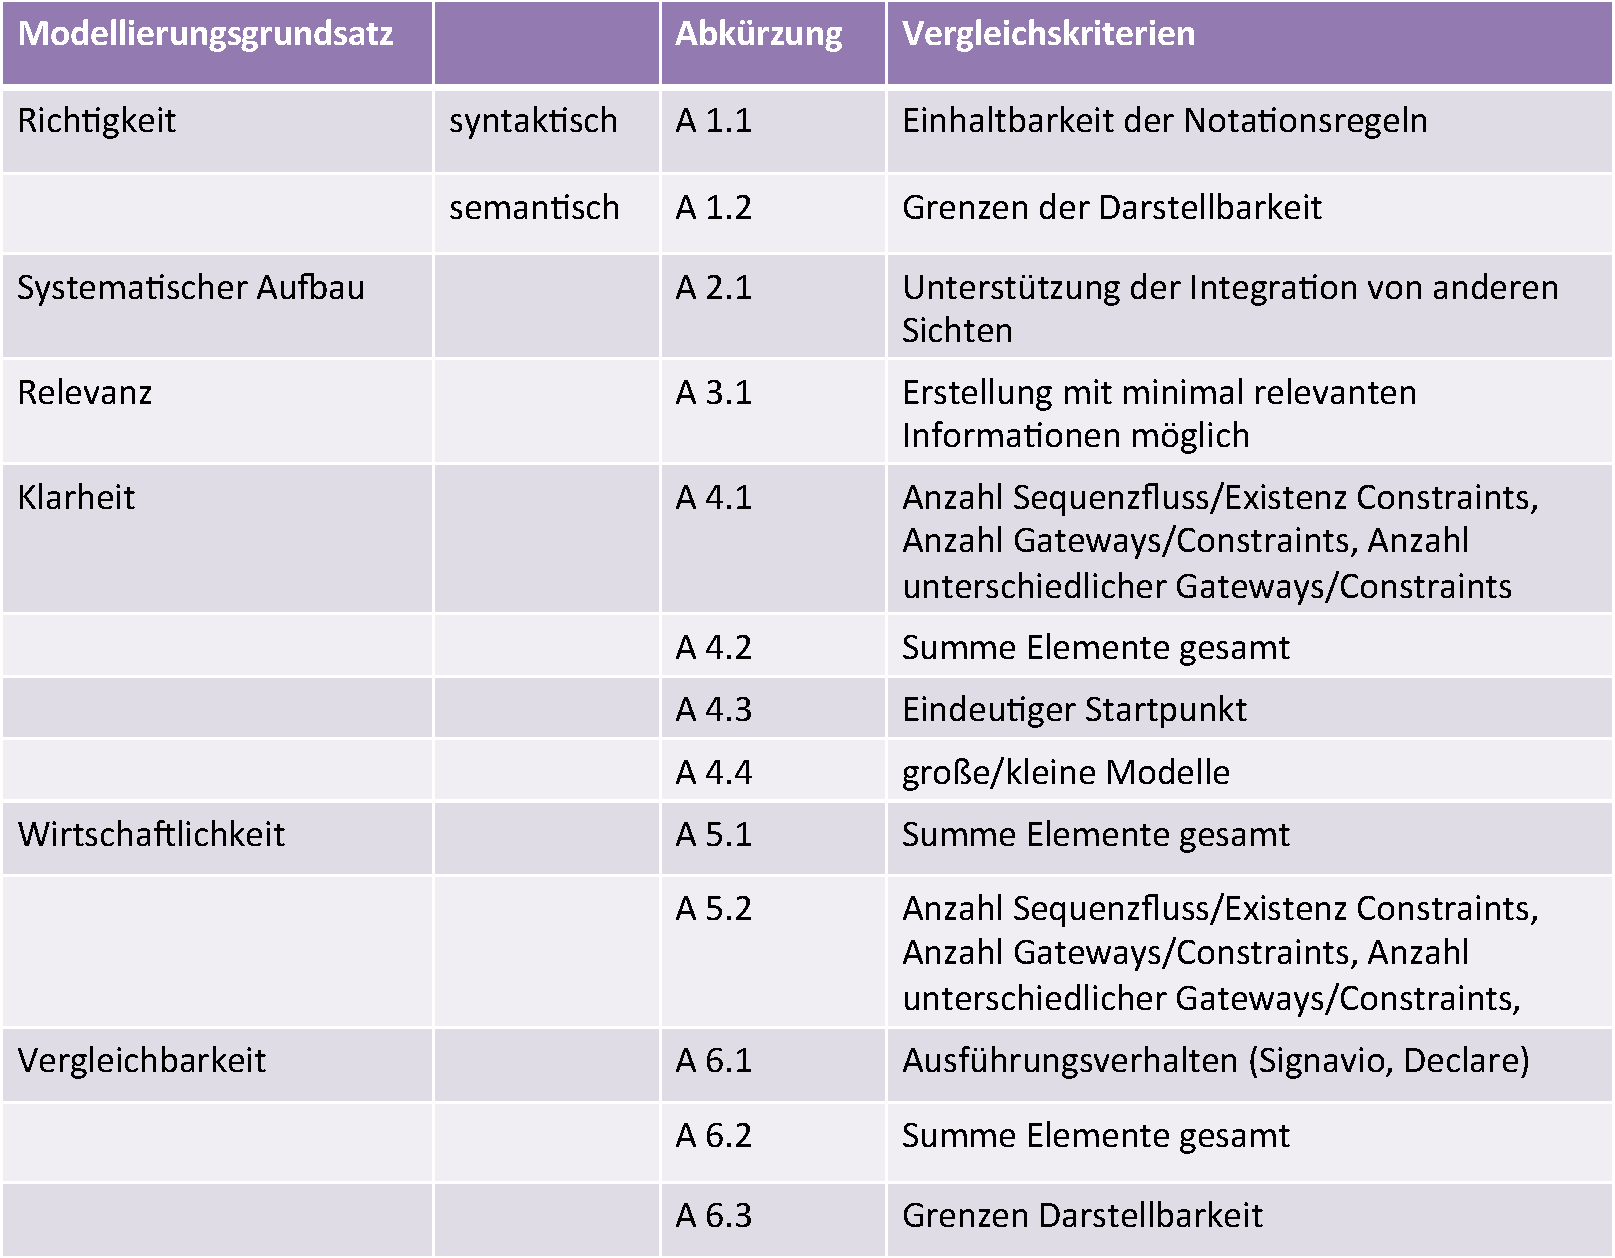
\includegraphics[width=\textwidth]{TabelleKriterien} %pdf, jpg, png...
  \caption{Übersicht Vergleichskriterien}
  \label{fig:TabelleKriterien}
\end{center}
\end{figure}








